\section{Experimental setup}
\label{sec:setup}

We aim to answer four questions:
\begin{enumerate}[nosep,leftmargin=*]
  \item How does accuracy change when every view is resized to one size?
  \item Which stages of the network need full resolution?
  \item Are the errors a model makes at different input sizes independent?
  \item How finely can the benchmark measure such differences?
\end{enumerate}

\paragraph{Models.}
We use the published weights of VGGT-1B~\cite{wang2025vggt} and \pithree~\cite{wang2025pi3} without fine-tuning. Both use $14{\times}14$ patches, a vision-transformer image encoder, and alternating frame and global attention with 2D rotary positions. VGGT treats its first view as a reference and uses a 518\,px input width by default; \pithree has no reference view. To run the probes, we reimplemented each model's forward pass as an explicit sequence of stages. Before every experiment, we verified in 32-bit precision that this decomposition reproduces the original model's outputs on real scenes (maximum absolute difference below $10^{-4}$). Experiments run in bfloat16 on a single GPU.

\begin{table}[t]
\centering\small
\setlength{\tabcolsep}{3pt}
\begin{adjustbox}{max width=\linewidth}
\begin{tabular}{@{}lcccc@{}}
\toprule
Probe & Pixels & Encoder & Frame att. & Global att. \\
\midrule
Full resolution        & full & full & full & full \\
Detail removed         & half$\uparrow$ & full & full & full \\
Encoder lowered        & half & half & full$^\dagger$ & full$^\dagger$ \\
Keys lowered           & full & full & full & keys half \\
Global lowered         & full & full & full & half$^\ddagger$ \\
All lowered            & half & half & half & half \\
\bottomrule
\end{tabular}
\end{adjustbox}
\caption{\textbf{Probes.} Each probe changes the resolution of one or more stages for 8 of the 12 views of a scene; the other 4 views stay at full resolution throughout. ``half$\uparrow$'': the image is reduced to half resolution and upsampled back, so the encoder receives a full-size image without its fine detail. $^\dagger$The encoder's half-resolution tokens are interpolated to the full grid. $^\ddagger$The views' tokens are pooled to half resolution before each global-attention block and the block's update is interpolated back; the prediction heads read these views at half resolution. All probes that use half-resolution positions map them onto the full-resolution grid.}
\label{tab:probes}
\end{table}

\begin{figure*}[t]
  \centering
  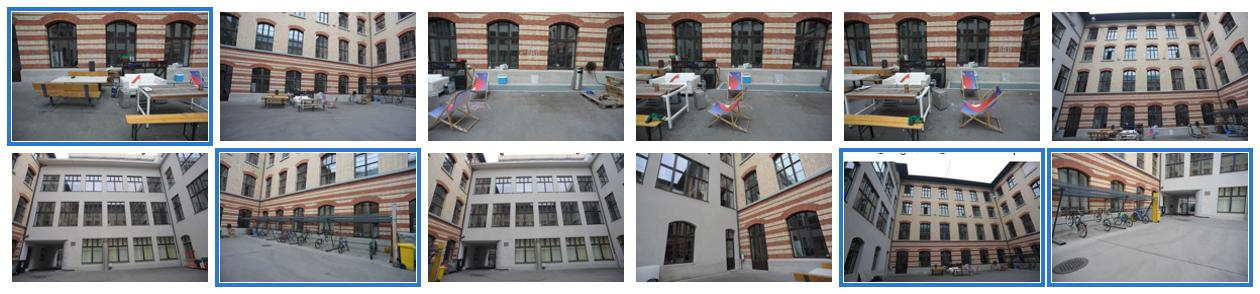
\includegraphics[width=\textwidth]{figures/fig_inputs.pdf}
  \caption{\textbf{The 12 input views of one ETH3D scene} (\emph{courtyard}), exactly as used in our ETH3D experiments, shown at reduced size. The 4 outlined views are the anchors, chosen by farthest-point sampling of the ground-truth camera centres; they stay at full resolution in every probe. The other 8 views are the ones whose processing each probe changes.}
  \label{fig:inputs}
\end{figure*}

\paragraph{Probes.}
Each scene gets 12 views. Four of them, chosen by farthest-point sampling of the ground-truth camera centres so that they spread over the scene, always stay at full resolution (\cref{fig:inputs}). These anchors give every probe the same full-resolution view of the scene's layout, so differences between probes come from how the other 8 views are processed. For the other 8 views, a probe lowers the resolution of specific stages by a factor of 2 per side (\cref{tab:probes}), which reduces their token count by about four and keeps every mapped position on an integer grid (\cref{eq:align}). \emph{Detail removed} keeps every stage at full resolution but feeds the encoder an image that has lost its fine detail; it measures whether the model uses pixel detail above half resolution. \emph{Encoder lowered} runs the encoder on the half-resolution image and interpolates its tokens to the full grid, so every later stage works at full resolution on coarser features. \emph{Keys lowered} keeps one query per full-resolution token in global attention but lets the other views read these 8 views only through keys and values area-pooled to the half-resolution grid; we add to the pooled keys' attention logits the logarithm of the number of full-resolution tokens each one replaces ($\log 3.83$ on 7-Scenes), so that a pooled key counts as the tokens it stands for. \emph{Global lowered} pools the queries as well. \emph{All lowered} runs every stage of these views at half resolution. Whenever a view's tokens sit on a half-resolution grid, we map their rotary positions onto the full-resolution grid,
\begin{equation}
  \tilde p \;=\; \rho\, p, \qquad \rho = 2,
  \label{eq:align}
\end{equation}
per axis, where $p$ is the zero-based patch index on the half-resolution grid; without this mapping, positions of the two grids disagree and accuracy drops further (\cref{sec:stages}).

\paragraph{Data.}
We use three datasets. On 7-Scenes~\cite{shotton2013scene} we draw 12 frames per scene at random from one sequence, with 10 independent draws for each of the 7 scenes (70 scene-draws); frames used during method development are excluded from these draws. Full resolution is $322{\times}420$ and half is $168{\times}210$. Its frames are small and quick to obtain, which let us repeat every probe on many draws; it is therefore the dataset on which we ran the most probes. ETH3D~\cite{schops2017eth3d} and HiRoom come from the benchmark release of Depth Anything~3~\cite{lin2025da3} and serve as a check that the findings do not depend on 7-Scenes. ETH3D has accurate laser-scanned ground truth; we use the 8 of its 11 scenes that have enough frames, at $294{\times}448$ and $154{\times}224$. For HiRoom we use the 19 of its 30 scenes that have at least 12 frames, at $364{\times}364$ and $182{\times}182$. On ETH3D and HiRoom our compute time allowed one draw of 12 frames per scene.

\paragraph{Metric and statistics.}
For every pair of views we compute the angular error of the predicted relative rotation and of the relative translation direction (ignoring its sign), take the larger of the two, and report the area under the cumulative error curve up to 3\textdegree{} (\auc) and 30\textdegree{} (\aucc), in percent. \auc rewards precise poses; \aucc rewards getting the layout roughly right. We integrate the exact empirical error distribution rather than a histogram, so absolute values are not directly comparable with numbers reported elsewhere. Differences between probes are paired by scene, and we give 95\% percentile intervals from 10{,}000 bootstrap resamples over scenes or scene-draws. We report intervals for the comparisons we computed them for, and means otherwise; a difference whose interval excludes zero is called significant. The supplementary material gives the implementation of every probe, all results in full, further probes, and the hypotheses we tested and rejected.
